\documentclass[12pt]{article}
\usepackage{graphicx}
\usepackage{hyperref}
\usepackage[letterpaper, portrait, margin=0.75in]{geometry}
\usepackage{fancyhdr}
\usepackage{pdfpages}
\usepackage{color}
\usepackage{multicol}
\usepackage{verbatim}
\usepackage{longtable}

\usepackage{charter}
\pagestyle{fancy}
\lhead{PSEC4A datasheet}
%\chead{\thepage}
\rhead{v0.2 ---  2017.5.9}

%%%%%%%%%%%%%%%%%%%%%%%%%
\usepackage{xparse} % NewDocumentCommand, IfValueTF, IFBooleanTF
\usepackage{tikz-timing}[2014/10/29]
\usetikztiminglibrary[rising arrows]{clockarrows}
%%%%%%%%%%%%%%%%%%%%%%%%%

%\usepackage{lmodern}

\NewDocumentCommand{\busref}{som}{\texttt{%
#3%
\IfValueTF{#2}{[#2]}{}%
\IfBooleanTF{#1}{\#}{}%
}}

\begin{document}
\noindent {\huge{\textbf {PSEC4A}}} \\
\noindent Chip Designer and Document Author: Eric Oberla (KICP UChicago) \\
\noindent Email: ejo@uchicago.edu

%\tableofcontents
%\newpage

\section*{Overview}
\begin{multicols}{2}

  This document provides an overview of the PSEC4A ASIC designed in late 2016 and early 2017 and submitted for fabrication on a MOSIS 0.13~$\mu$m CMOS MPW in February, 2017. The PSEC4A ASIC is intended for the `analog down-conversion' of wide-bandwidth ($\sim$2~GHz) analog signals, achieved through fast sampling (1-11 gigasamples-per-second [GSPS]) followed by a relatively slow digitization and readout process ($\mathcal{O}$100~MHz). Thus, PSEC4A requires a trigger signal to capture the signal-of-interest, either from an external source or generated using the PSEC4A internal discriminators.

  The PSEC4A has 8 signal input channels. Each channel has 1056 samples, which are randomly addressable in blocks of 132 samples. The sampling rate is set by an external clock input, which is locked on-chip using a delay-locked loop (DLL). When successfully locked, one input clock period spans the primary sampling array and the sampling rate is equal to 132*$f$, where $f$ is the input clock frequency.
  
\end{multicols}

\section*{Features}
\begin{itemize}
{\bf
  \item `Fast' and `Slow' DLL modes to allow a wide range of stable sampling rates, from $\sim$1~GSPS to 11~GSPS.
  \item Improved input coupling to extend analog bandwidth
  \item Simultaneous sampling / digitization / readout functionality to reduce dead-time induced latency
  \item Multi-buffering via addressable switched-capacitor banks.
  \item On-chip 10-bit DACs for biases and thresholds
  \item Each channel with a threshold-level discriminator and trigger output pin
  \item 11-bit ramp-compare ADC using on-chip 1.5~GHz clock generator
  \item Can be powered through a single 1.2V supply
}

    
\end{itemize}

\section*{Absolute Maximum ratings}
\begin{center}
\begin{tabular}[b!]{l|p{1.4cm}|p{1.7cm}|p{9cm}}
  \hline
   spec       & max & nominal & comment \\ \hline
   Supply Voltage ($\mathrm{V_{dd}}$) &  1.5 V  & 1.2 V  &   may be possible to increase $\mathrm{AV_{dd}}$ only to increase dynamic range\\ \hline
   IO voltage &  $\mathrm{V_{dd}}$ & 1.2 V & Over/under voltage protection diodes on most pins. ({\bf Not} on signal inputs) \\ \hline
   Signal range voltage & 0-$\mathrm{AV_{dd}}$ & 0.1-1.1~V & about a 1~V usable range

\end{tabular}
\end{center}

\newpage
\section*{I/O Descriptions}
The PSEC4A pinout, as housed in the LQFP128 package, is shown in Figure~\ref{fig:pinout}.

\begin{figure}[t!]
    \begin{center}
      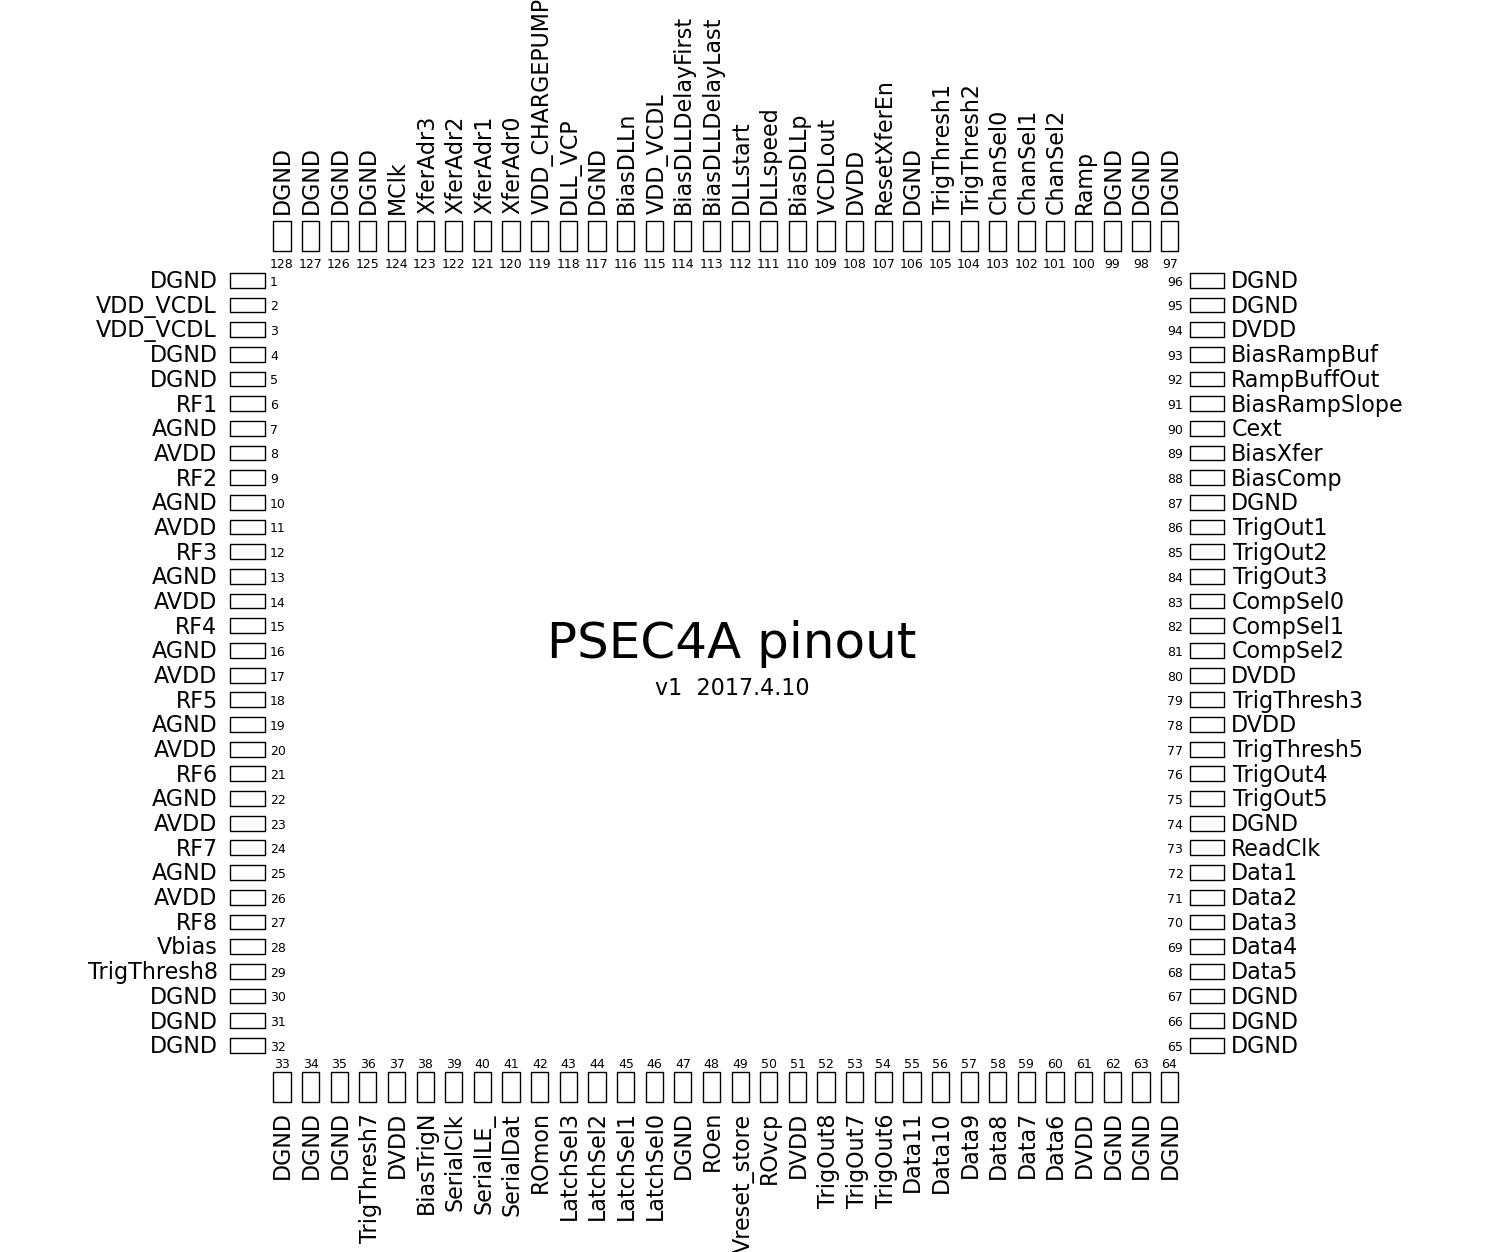
\includegraphics[width=18.5cm]{fig/PSEC4a_pinout_LQFP128.png}
      %\includegraphics[width=15cm]{singlePLL.PNG}

    \end{center}
    \caption{PSEC4A pinout in LQFP128 package}
    \label{fig:pinout}
\end{figure}

\subsection*{Power}
The PSEC4A has four separate +1.2~V $\mathrm{V_{dd}}$ rails and two GND returns.
These can be tied to a single power supply (+1.2~V, GND), but there may (potentially) be
performance benefits when taking care to provide some isolation between these rails. 

\begin{center}
\begin{tabular}[h!]{l|l|p{10cm}}
  \hline
   power rail       & ref &  comment \\ \hline \hline
   $\mathrm{DV_{dd}}$ &  DGND  &  power rail for digital circuitry  \\ \hline
   $\mathrm{V_{dd}VCDL}$ &  DGND  &  power rail for timing generation circuits (VCDL and chip-wide timing drivers) \\ \hline
   $\mathrm{V_{dd}ChargePump}$ &  DGND  &  power rail for DLL feedback circuit \\ \hline
   $\mathrm{AV_{dd}}$ &  AGND  &  power rail for analog circuits and DACs \\ \hline

\end{tabular}
\end{center}

It is likely that using a single PCB GND plane for both DGND and AGND will be satisfactory.

For a conservative design, it is suggested that: 

1) $\mathrm{AV_{dd}}$ be generated by a separate regulator

2) $\mathrm{V_{dd}VCDL}$ be isolated from the $\mathrm{DV_{dd}}$ plane using an appropriate ferrite.

3) $\mathrm{V_{dd}ChargePump}$ be independently generated or further isolated from  $\mathrm{V_{dd}VCDL}$ using a ferrite.
$\mathrm{V_{dd}ChargePump}$ should draw no more than a couple mA.

\subsection*{Digital I/0s}

\begin{center}
\begin{longtable}[h!]{|l|l|l| p{11cm}|}
  \hline
   pin \# & pin name & type & description\\ \hline \hline
   39 & SerialClk & IN & clock for serial interface \\ \hline
   40 & SerialLE\_ & IN & Load signal (active low) for serial interface\\ \hline
   41 & SerialDat & IN & data line for serial interface\\ \hline
   43 & LatchSel3 & IN & Internal latch select decoder, bit 3 (MSB)\\ \hline
   44 & LatchSel2 & IN & Internal latch select decoder, bit 2 \\ \hline
   45 & LatchSel1 & IN & Internal latch select decoder, bit 1 \\ \hline
   46 & LatchSel0 & IN & Internal latch select decoder, bit 0 (LSB)\\ \hline
   45 & ROen & IN & Enable fanout buffers for ring oscillator chip-wide ADC clock \\ \hline
   52 & TrigOut8 & OUT & Trigger bit output on channel 8 (may be left open if not using self trigger)\\ \hline
   53 & TrigOut7 & OUT & Trigger bit output on channel 7 (may be left open if not using self trigger)\\ \hline
   54 & TrigOut6 & OUT & Trigger bit output on channel 6 (may be left open if not using self trigger)\\ \hline
   55 & DataOut11 & OUT & ADC data\\ \hline
   56 & DataOut10 & OUT & ADC data\\ \hline
   57 & DataOut9 & OUT & ADC data\\ \hline
   58 & DataOut8 & OUT & ADC data\\ \hline
   59 & DataOut7 & OUT & ADC data\\ \hline
   60 & DataOut6 & OUT & ADC data\\ \hline
   68 & DataOut5 & OUT & ADC data\\ \hline
   69 & DataOut4 & OUT & ADC data\\ \hline
   70 & DataOut3 & OUT & ADC data\\ \hline
   71 & DataOut2 & OUT & ADC data\\ \hline
   72 & DataOut1 & OUT & ADC data\\ \hline
   73 & ReadClk  & IN & Clock for data readout\\ \hline
   75 & TrigOut5 & OUT & Trigger bit output on channel 5 (may be left open if not using self trigger)\\ \hline
   76 & TrigOut4 & OUT & Trigger bit output on channel 4 (may be left open if not using self trigger)\\ \hline
   81 & CompSel2 & IN & Internal comparator select decoder, bit 2 (MSB) \\ \hline
   82 & CompSel1 & IN & Internal comparator select decoder, bit 1 \\ \hline
   83 & CompSel0 & IN & Internal comparator select decoder, bit 0 (LSB)\\ \hline  
   84 & TrigOut3 & OUT & Trigger bit output on channel 3 (may be left open if not using self trigger)\\ \hline
   85 & TrigOut2 & OUT & Trigger bit output on channel 2 (may be left open if not using self trigger)\\ \hline
   86 & TrigOut1 & OUT & Trigger bit output on channel 1 or the OR of all 8 trigger outputs as selected in the Serial Interface (may be left open if not using self trigger)\\ \hline
   100 & Ramp & IN & Start ADC ramp \\ \hline
   101 & ChanSel2 & IN & Internal channel select decoder, bit 2 (MSB) \\ \hline
   102 & ChanSel1 & IN & Internal channel select decoder, bit 1 \\ \hline
   103 & ChanSel0 & IN & Internal channel select decoder, bit 0 (LSB)\\ \hline
   107 & ResetXferEn & INOUT & Enable or disable the reset stage of the analog storage caps. Nominally set in the Serial Interface. \\ \hline
   109 & VCDLout & OUT & Delayed-by-148 samples MClk output (primarly for debugging) \\ \hline
   111 & DLLspeed & INOUT & Pick fast or slow DLL mode. Nominally set in the Serial Interface. \\ \hline
   112 & DLLstart & IN & Reset/start DLL \\ \hline
   120 & XferAdr0 & IN & Internal analog transfer address decoder, bit 0 (LSB)\\ \hline
   121 & XferAdr1 & IN & Internal analog transfer address decoder, bit 1 \\ \hline
   122 & XferAdr2 & IN & Internal analog transfer address decoder, bit 2 \\ \hline
   123 & XferAdr3 & IN & Internal analog transfer address decoder, bit 3 (MSB)\\ \hline
   124 & MClk & IN & Sampling clock \\ \hline
   
\end{longtable}
\end{center}

\begin{comment}
\subsection*{Serial Interface}

\begin{tikztimingtable}[%
    timing/dslope=0.4,
    timing/.style={x=5ex,y=2ex},
    x=3ex,
    timing/rowdist=4ex,
    timing/c/rising arrows,
    timing/name/.style={font=\sffamily\scriptsize},
  ]
\busref{CLK} &  U8{C}H\\
\busref{data} & Hhh2D{msb};[dotted] 2D{};  2D{lsb}LH\\
\end{tikztimingtable}

\begin{tikztimingtable}[%
    timing/dslope=0.1,
    timing/.style={x=5ex,y=2ex},
    x=5ex,
    timing/rowdist=3ex,
    timing/name/.style={font=\sffamily\scriptsize}
]
\busref{CLK}         & 10{C} \\
\busref*{FRAME}      & U h l L l h 4H 2U \\
\busref[31::0]{AD}   & U u 2X 2.5U 2D{$v_i$} 2U \\
\busref*[3::0]{C/BE} & U u 2D{0000} 4.5D{\busref*{BE}} 2U  \\
\busref*{IRDY}       & 3.5U 4.5L 2H \\
\busref*{TRDY}       & 3.5U 2.5H 2L 2H \\
\busref*{DEVSEL}     & 5U hl 2L h 1.5U \\
\extracode
\begin{pgfonlayer}{background}
\begin{scope}[semitransparent ,semithick]
\vertlines[darkgray,dotted]{1.0,3.0,...,9.0}
\vertlines[gray,dotted]{2.0,4.0,...,8.0}
\end{scope}
\end{pgfonlayer}
\end{tikztimingtable}

\begin{tikztimingtable}[%
    timing/dslope=0.4,
    timing/.style={x=5ex,y=2ex},
    x=3ex,
    timing/rowdist=4ex,
    timing/c/rising arrows,
    timing/name/.style={font=\sffamily\scriptsize},
]
\busref{CLK}  &  U8{C}H\\
\busref{data} & Hhh2D{msb};[dotted] 2D{};  2D{lsb}LH\\
\end{tikztimingtable}

\begin{figure}[h!]
    \begin{center}
      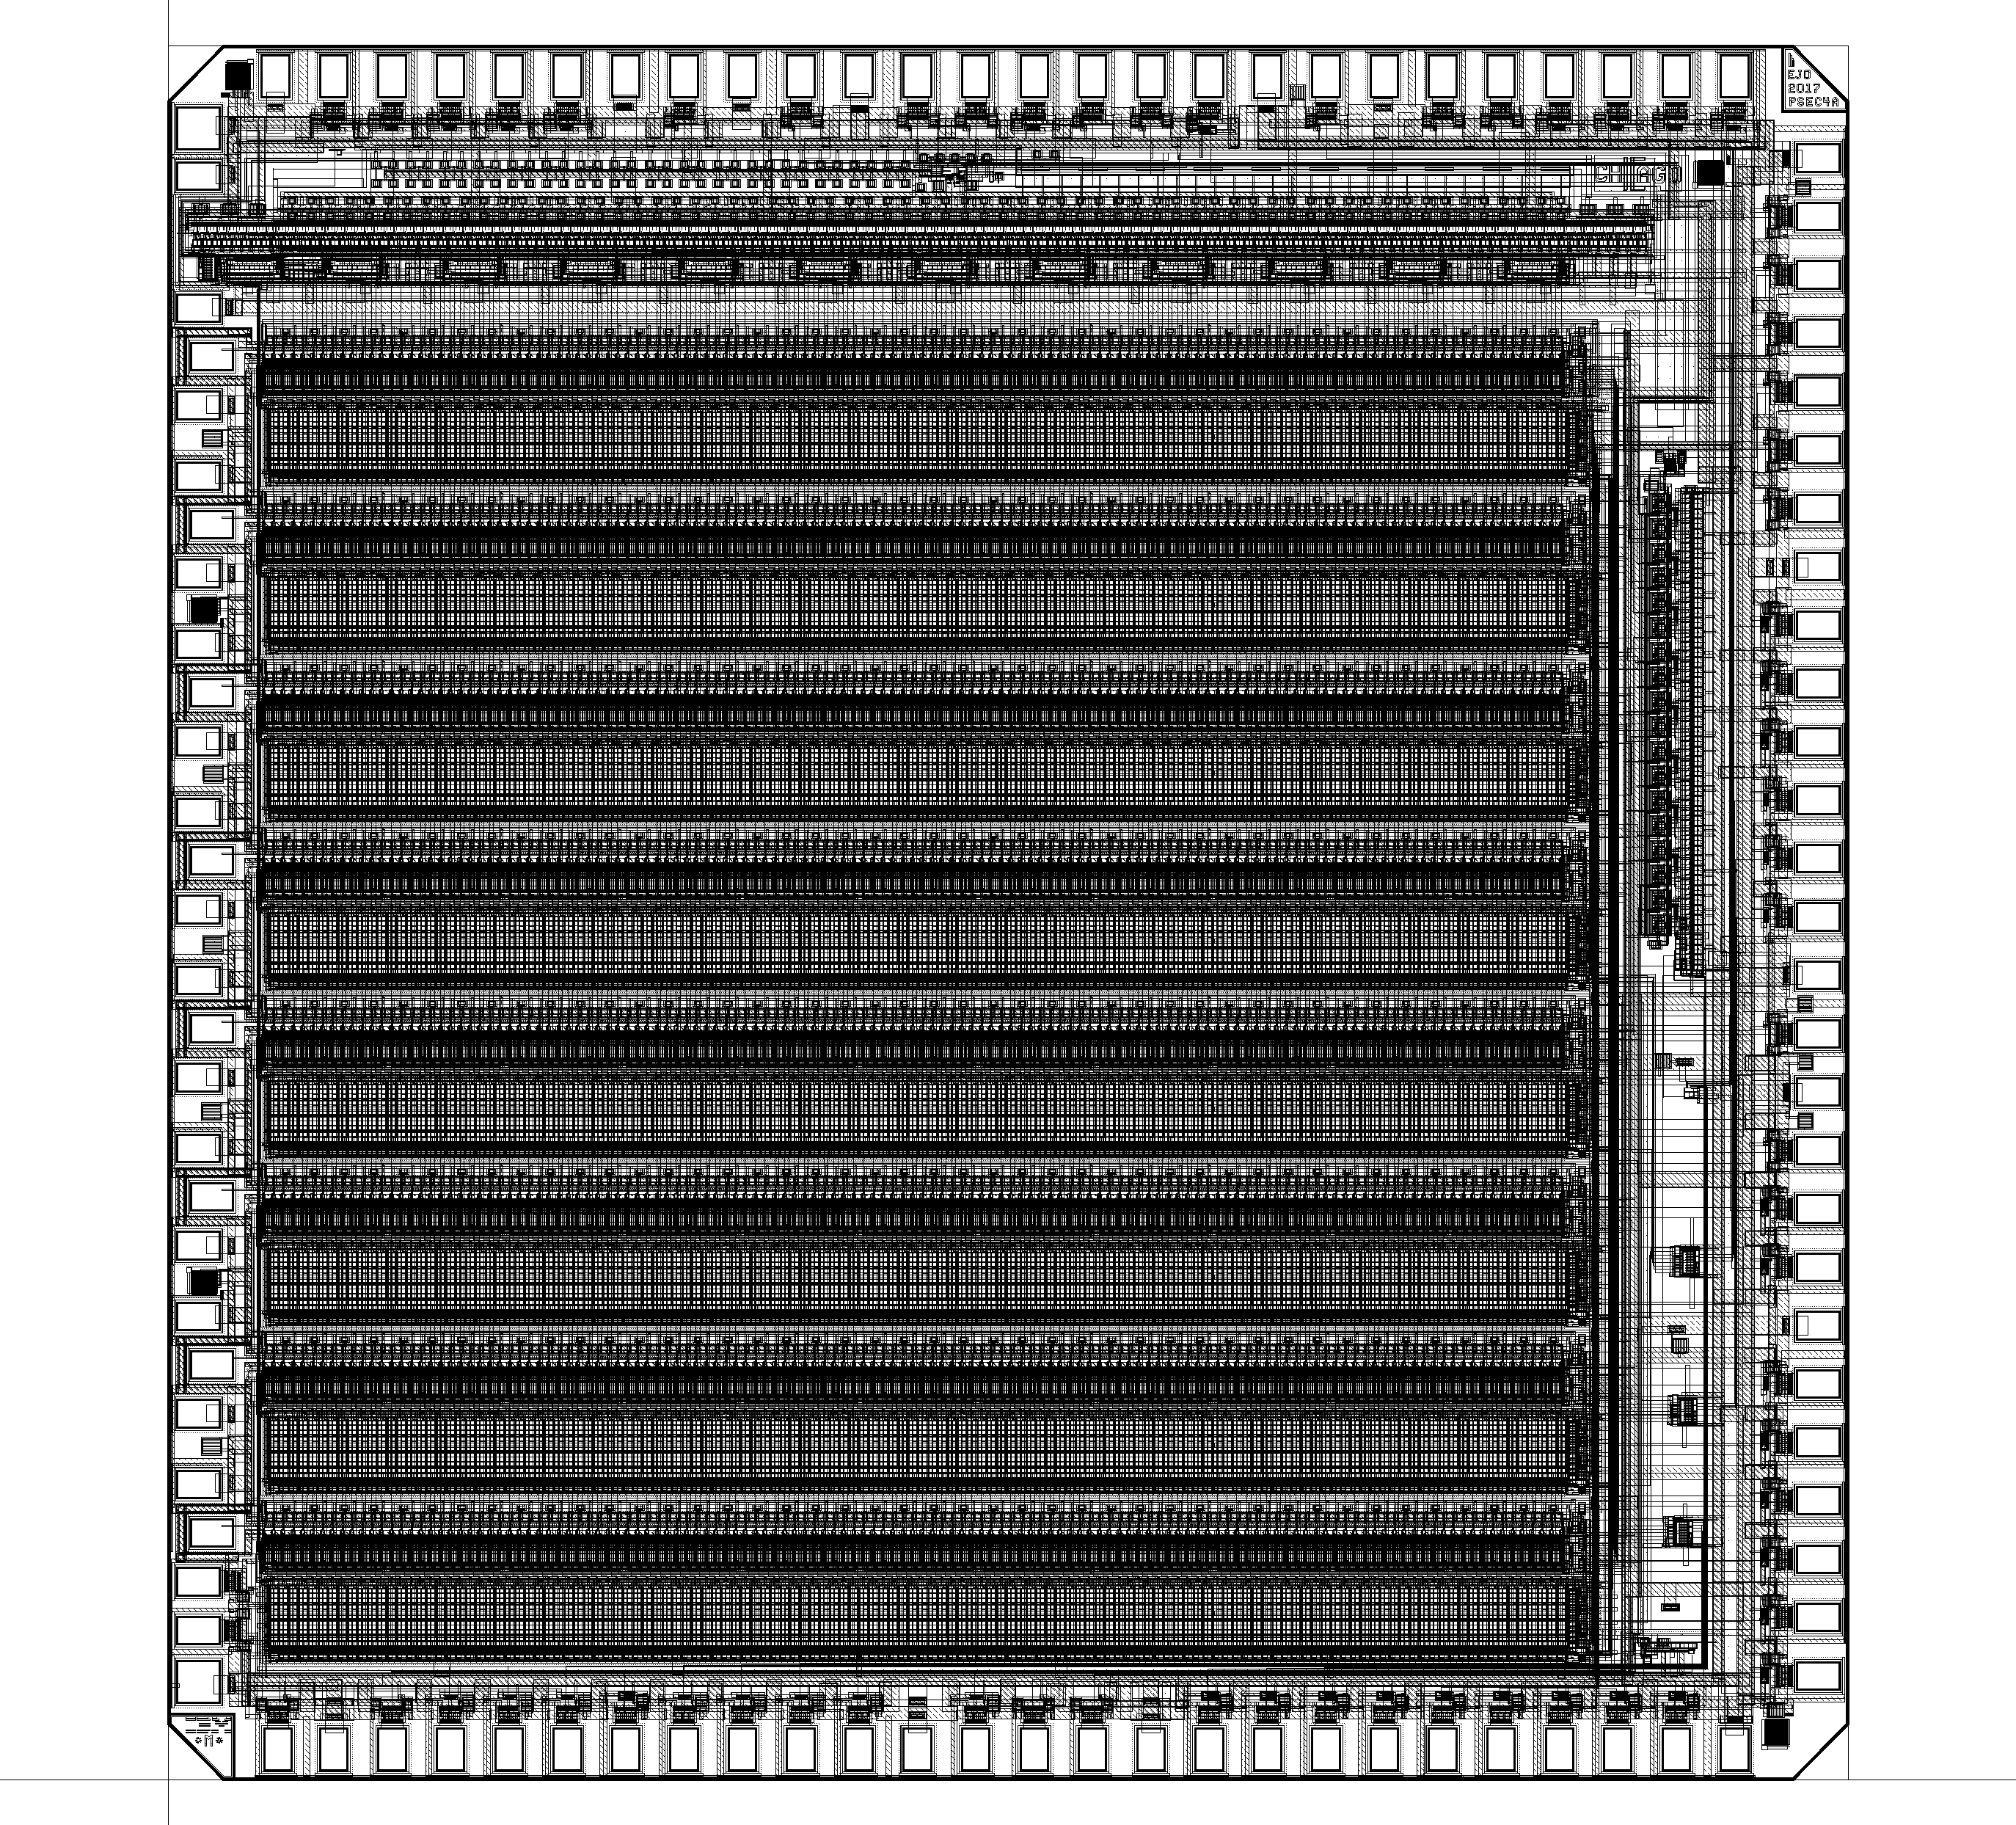
\includegraphics[width=17.5cm]{fig/psec4a_layout_capture}
      %\includegraphics[width=15cm]{singlePLL.PNG}

    \end{center}
    \caption{PSEC4a black-and-white layout capture. The die has 107 pads. The layout has an area of 3800 $\times$ 3920~$\mu$$m^2$.}
    \label{fig:layout}
\end{figure}

\end{comment}

\subsection*{Analog I/0s}

\subsubsection*{RF inputs}
\begin{itemize}
\item Pins 6,9,12,15,18,21,24,27 are signal inputs 1 through 8, respectively. 
\item These are not ESD protected. 
\item Each signal line should be terminated with the appropriate impedance (typically a 50 ohm 0402 resistor) as close as possible to these inputs. 
\item Each signal line should be AC coupled before this termination and a DC pedestal bias (between 0.2 and 1.0V) should be applied to the signal-return side of the
  termination resistor or inductor.
\end{itemize}

\subsubsection*{PSEC4A DAC debugging outputs}
Most of the analog biases required to run the chip can be generated on-chip with 17 digital-to-analog converters (DAC) that are programmed
through the Serial Interface.
The DC voltages of most of these DACs are sent to external pads for debugging purposes. If issues arise with the PSEC4A DAC design or Serial Interface,
these DAC pins may be over-ridden using a low-impedance buffer amplifier.

This also allows additional decoupling
capacitors to be added to these analog levels,if necessary.

The PSEC4A DACs and associated package pins, if applicable, are listed in the following table:

\begin{center}
\begin{longtable}[h!]{|l|l|l| p{10.5cm}|}
  \hline
  DAC \# & DAC/pin name & pin \# & description\\ \hline \hline
  1 & ROvcp & 50 & Bias voltage for ring oscillator clock speed (V=0 fastest) \\ \hline
  2 & BiasTrigN & 38 & Bias voltage for self-trigger discrimators (V=1.2 max current bias) \\ \hline
  3 & BiasXfer & 89 & Bias voltage for analog transfer buffer \\ \hline
  4 & BiasRampBuf & 93 & Bias voltage for ramp buffer in each cell \\ \hline
  5 & BiasComp & 88 & Bias voltage for ADC comparators \\ \hline
  6 & BiasDllDelayLast & 113 & Delay tuning for last timing cell \\ \hline
  7 & BiasDllDelayLast & 114 & Delay tuning for first sample cell \footnote{together with BiasDLLDelayLast, this allows the wraparound sample (sample 132 back to sample 1 in the primary sampling array) to be tuned to a specific duration} \\ \hline
  8 & BiasDLLp & 110 & Tuning voltage for DLL pFET charge pump current \\ \hline
  9 & BiasDLLn & 116 & Tuning voltage for DLL nFET charge pump current \\ \hline
  10 & TrigThresh1 & 105 & Trigger threshold voltage for channel 1 \\ \hline
  11 & TrigThresh2 & 104 & Trigger threshold voltage for channel 2 \\ \hline
  12 & TrigThresh3 & 79  & Trigger threshold voltage for channel 3 \\ \hline
  13 & TrigThresh4 & -- & Trigger threshold voltage for channel 4 \\ \hline
  14 & TrigThresh5 & 77  & Trigger threshold voltage for channel 5 \\ \hline
  15 & TrigThresh6 & -- & Trigger threshold voltage for channel 6 \\ \hline
  16 & TrigThresh7 & 36  & Trigger threshold voltage for channel 7 \\ \hline
  17 & TrigThresh8 & 29  & Trigger threshold voltage for channel 8 \\ \hline
  18 & BiasRampSlope & 91 & Bias voltage to tune the ADC ramp slope \\ \hline
\end{longtable}
\end{center}
   

%\clearpage
%
%\appendix
%
%\includepdf[pages={1},  offset=0cm -6cm, pagecommand={\section{IPython Notebook: Startup}\label{Appendix0}}]{fig/bootSurf_notebook.pdf}
%\includepdf[pages=2-, offset=0cm -1cm, pagecommand={}]{fig/bootSurf_notebook.pdf}
%
%\includepdf[pages={1}, offset=0cm -2cm, pagecommand={\section{IPython Notebook: Basic Operations}\label{Appendix1}}]{fig/surf_ipython.pdf}
%\includepdf[pages=2-, offset=0cm -2cm, pagecommand={}]{fig/surf_ipython.pdf}
%
%\includepdf[pages={1}, offset=0cm -1cm, pagecommand={\section{IPython Notebook: Tuning DLL feedback trim}\label{Appendix2}}]{fig/vtrimfb_notebook.pdf}
%\includepdf[pages={2-}, offset=0cm -1cm, pagecommand={}]{fig/vtrimfb_notebook.pdf}
%
\end{document}
